% ============================================================
%  PROBLEM 1 — worked example
%  Shows: a multi-step derivation, \cref chains between equations,
%         single figures, a small table, and a citation.
% ============================================================

\section*{Problem 1}
\phantomsection
\addcontentsline{toc}{section}{Problem 1}   % ← registers it for bookmarks

\subsection*{Task a)}
\phantomsection
\addcontentsline{toc}{subsection}{Task a)}

The task is to study the cardinal sine, or \emph{sinc} function, and to locate
its zeros and its extrema. The function is defined as

\begin{equation} \label{sinc}
	f(x) = \frac{\sin x}{x} \; \; \; \text{, defined for } x \neq 0
\end{equation}

\Cref{sinc} is undefined at the origin, but the singularity is removable. The
Maclaurin series of the numerator gives

\begin{equation} \label{series}
	\sin x = x - \frac{x^3}{3!} + \frac{x^5}{5!} - \dots
	\; \; \Rightarrow \; \;
	\frac{\sin x}{x} = 1 - \frac{x^2}{6} + \frac{x^4}{120} - \dots
\end{equation}

so that $\displaystyle\lim_{x \to 0} f(x) = 1$, and the function is made
continuous everywhere by defining $f(0) := 1$. The right-hand side of
\cref{series} is even, which is the first thing to note about the shape: the
curve is symmetric about the vertical axis.

The zeros follow directly from \cref{sinc}. Since the denominator never
vanishes on the domain, $f(x) = 0$ exactly when $\sin x = 0$:

\begin{equation} \label{zeros}
	f(x) = 0 \; \; \Leftrightarrow \; \; x = n\pi \; \; \; \text{, } n \in \mathbb{Z} \setminus \{0\}
\end{equation}

The extrema are less convenient. Differentiating \cref{sinc} with the quotient
rule and setting the result to zero gives

\begin{equation} \label{extrema}
	f'(x) = \frac{x\cos x - \sin x}{x^2} = 0
	\; \; \Rightarrow \; \;
	\tan x = x
\end{equation}

\Cref{extrema} is transcendental and has no closed-form solution, so the
turning points have to be found numerically. Newton's method applied to
$g(x) = \tan x - x$ converges in a handful of iterations from a starting point
near each $(n + \nicefrac{1}{2})\pi$; the same method is treated properly in
Problem 3. The first few roots and the function values there are collected in
\cref{tab:extrema}.

\begin{table}[htbp]
	\centering
	\caption{Location of the first extrema of \cref{sinc}, obtained by solving
	\cref{extrema} numerically to six decimals.}
	\label{tab:extrema}
	\begin{tabular}{|c|c|c|}
		\hline
		$n$ & $x_n$ & $f(x_n)$ \\
		\hline
		0 & 0.000000 & \phantom{-}1.000000 \\
		\hline
		1 & 4.493409 & -0.217234 \\
		\hline
		2 & 7.725252 & \phantom{-}0.128375 \\
		\hline
		3 & 10.904122 & -0.091325 \\
		\hline
	\end{tabular}
\end{table}

The envelope of those values decays like $1/x$, which is visible in
\cref{fig:sinc}: the central lobe reaches $1$, the first side lobe only reaches
about $22\%$ of that, and the decay continues from there.

\begin{figure}[htbp]
	\centering
	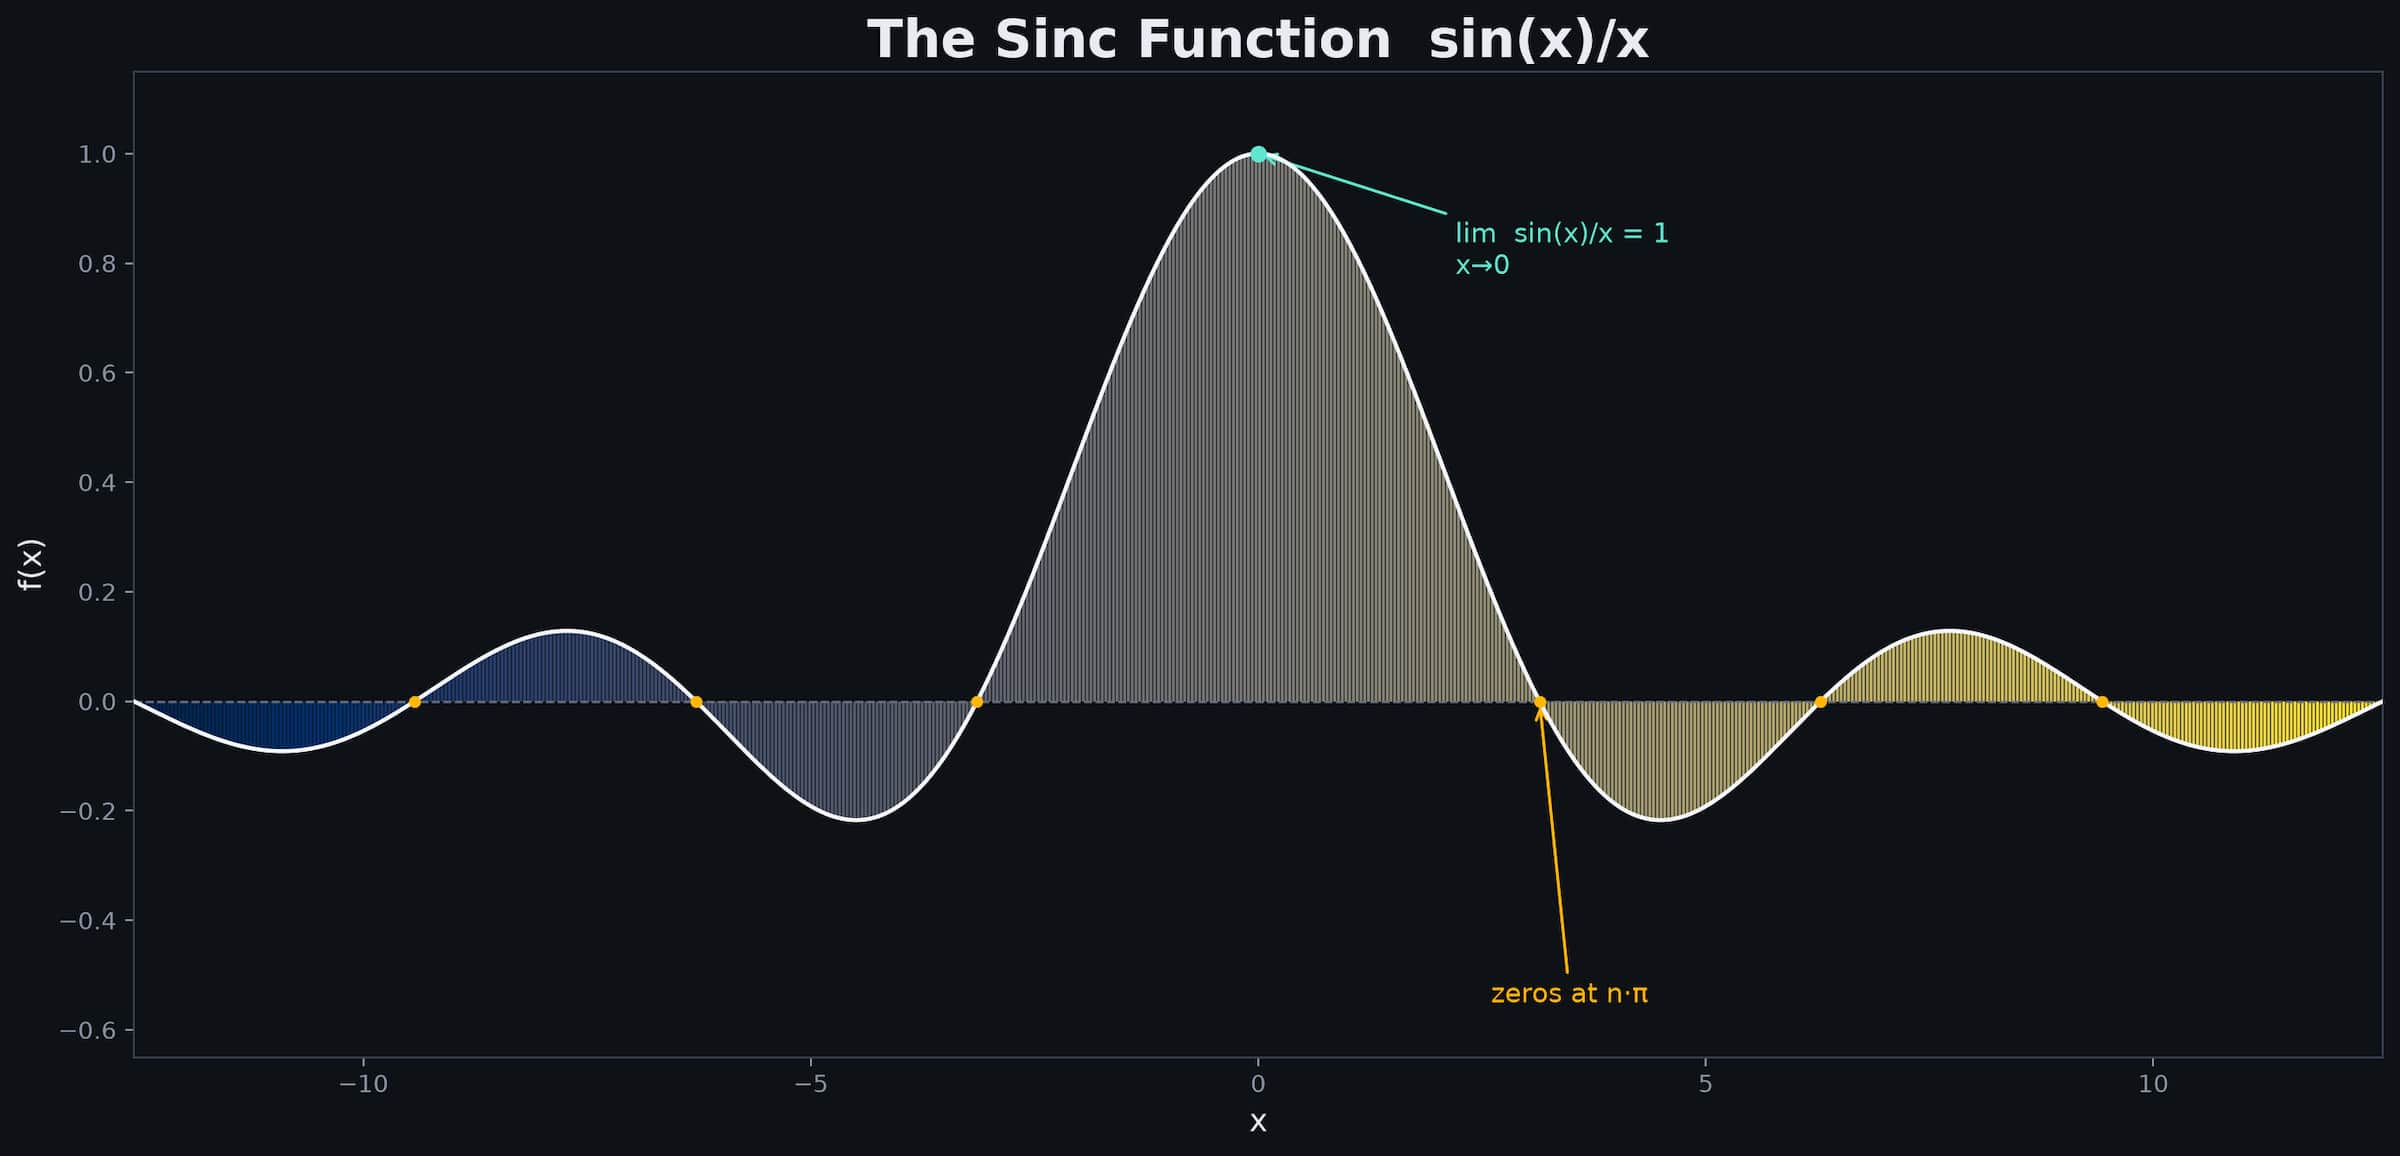
\includegraphics[width=0.95\linewidth]{graphs/sinc_fill}
	\caption{The sinc function of \cref{sinc} over $x \in [-13, 13]$, with the
	area under the curve shaded. The zeros marked on the axis are the ones
	predicted by \cref{zeros}, and the annotated limit at the origin is the one
	derived in \cref{series}.}
	\label{fig:sinc}
\end{figure}

\FloatBarrier

\subsection*{Task b)}
\phantomsection
\addcontentsline{toc}{subsection}{Task b)}

The task is to extend \cref{sinc} to two dimensions and to describe the
resulting surface. Replacing the argument with the radial distance
$r = \sqrt{x^2 + y^2}$ gives the radially symmetric function

\begin{equation} \label{sombrero}
	z(x,y) = \frac{\sin r}{r} \; \; \; \text{, } r = \sqrt{x^2+y^2}
\end{equation}

Because \cref{sombrero} depends on $x$ and $y$ only through $r$, every
property derived in Task a) carries over as a property of a circle rather than
of a point. The zeros of \cref{zeros} become concentric rings of radius
$r = n\pi$, the maximum $z = 1$ sits at the single point $r = 0$, and the
extrema of \cref{tab:extrema} become circular ridges and troughs. The
resulting surface is plotted in \cref{fig:sombrero}.

\begin{figure}[htbp]
	\centering
	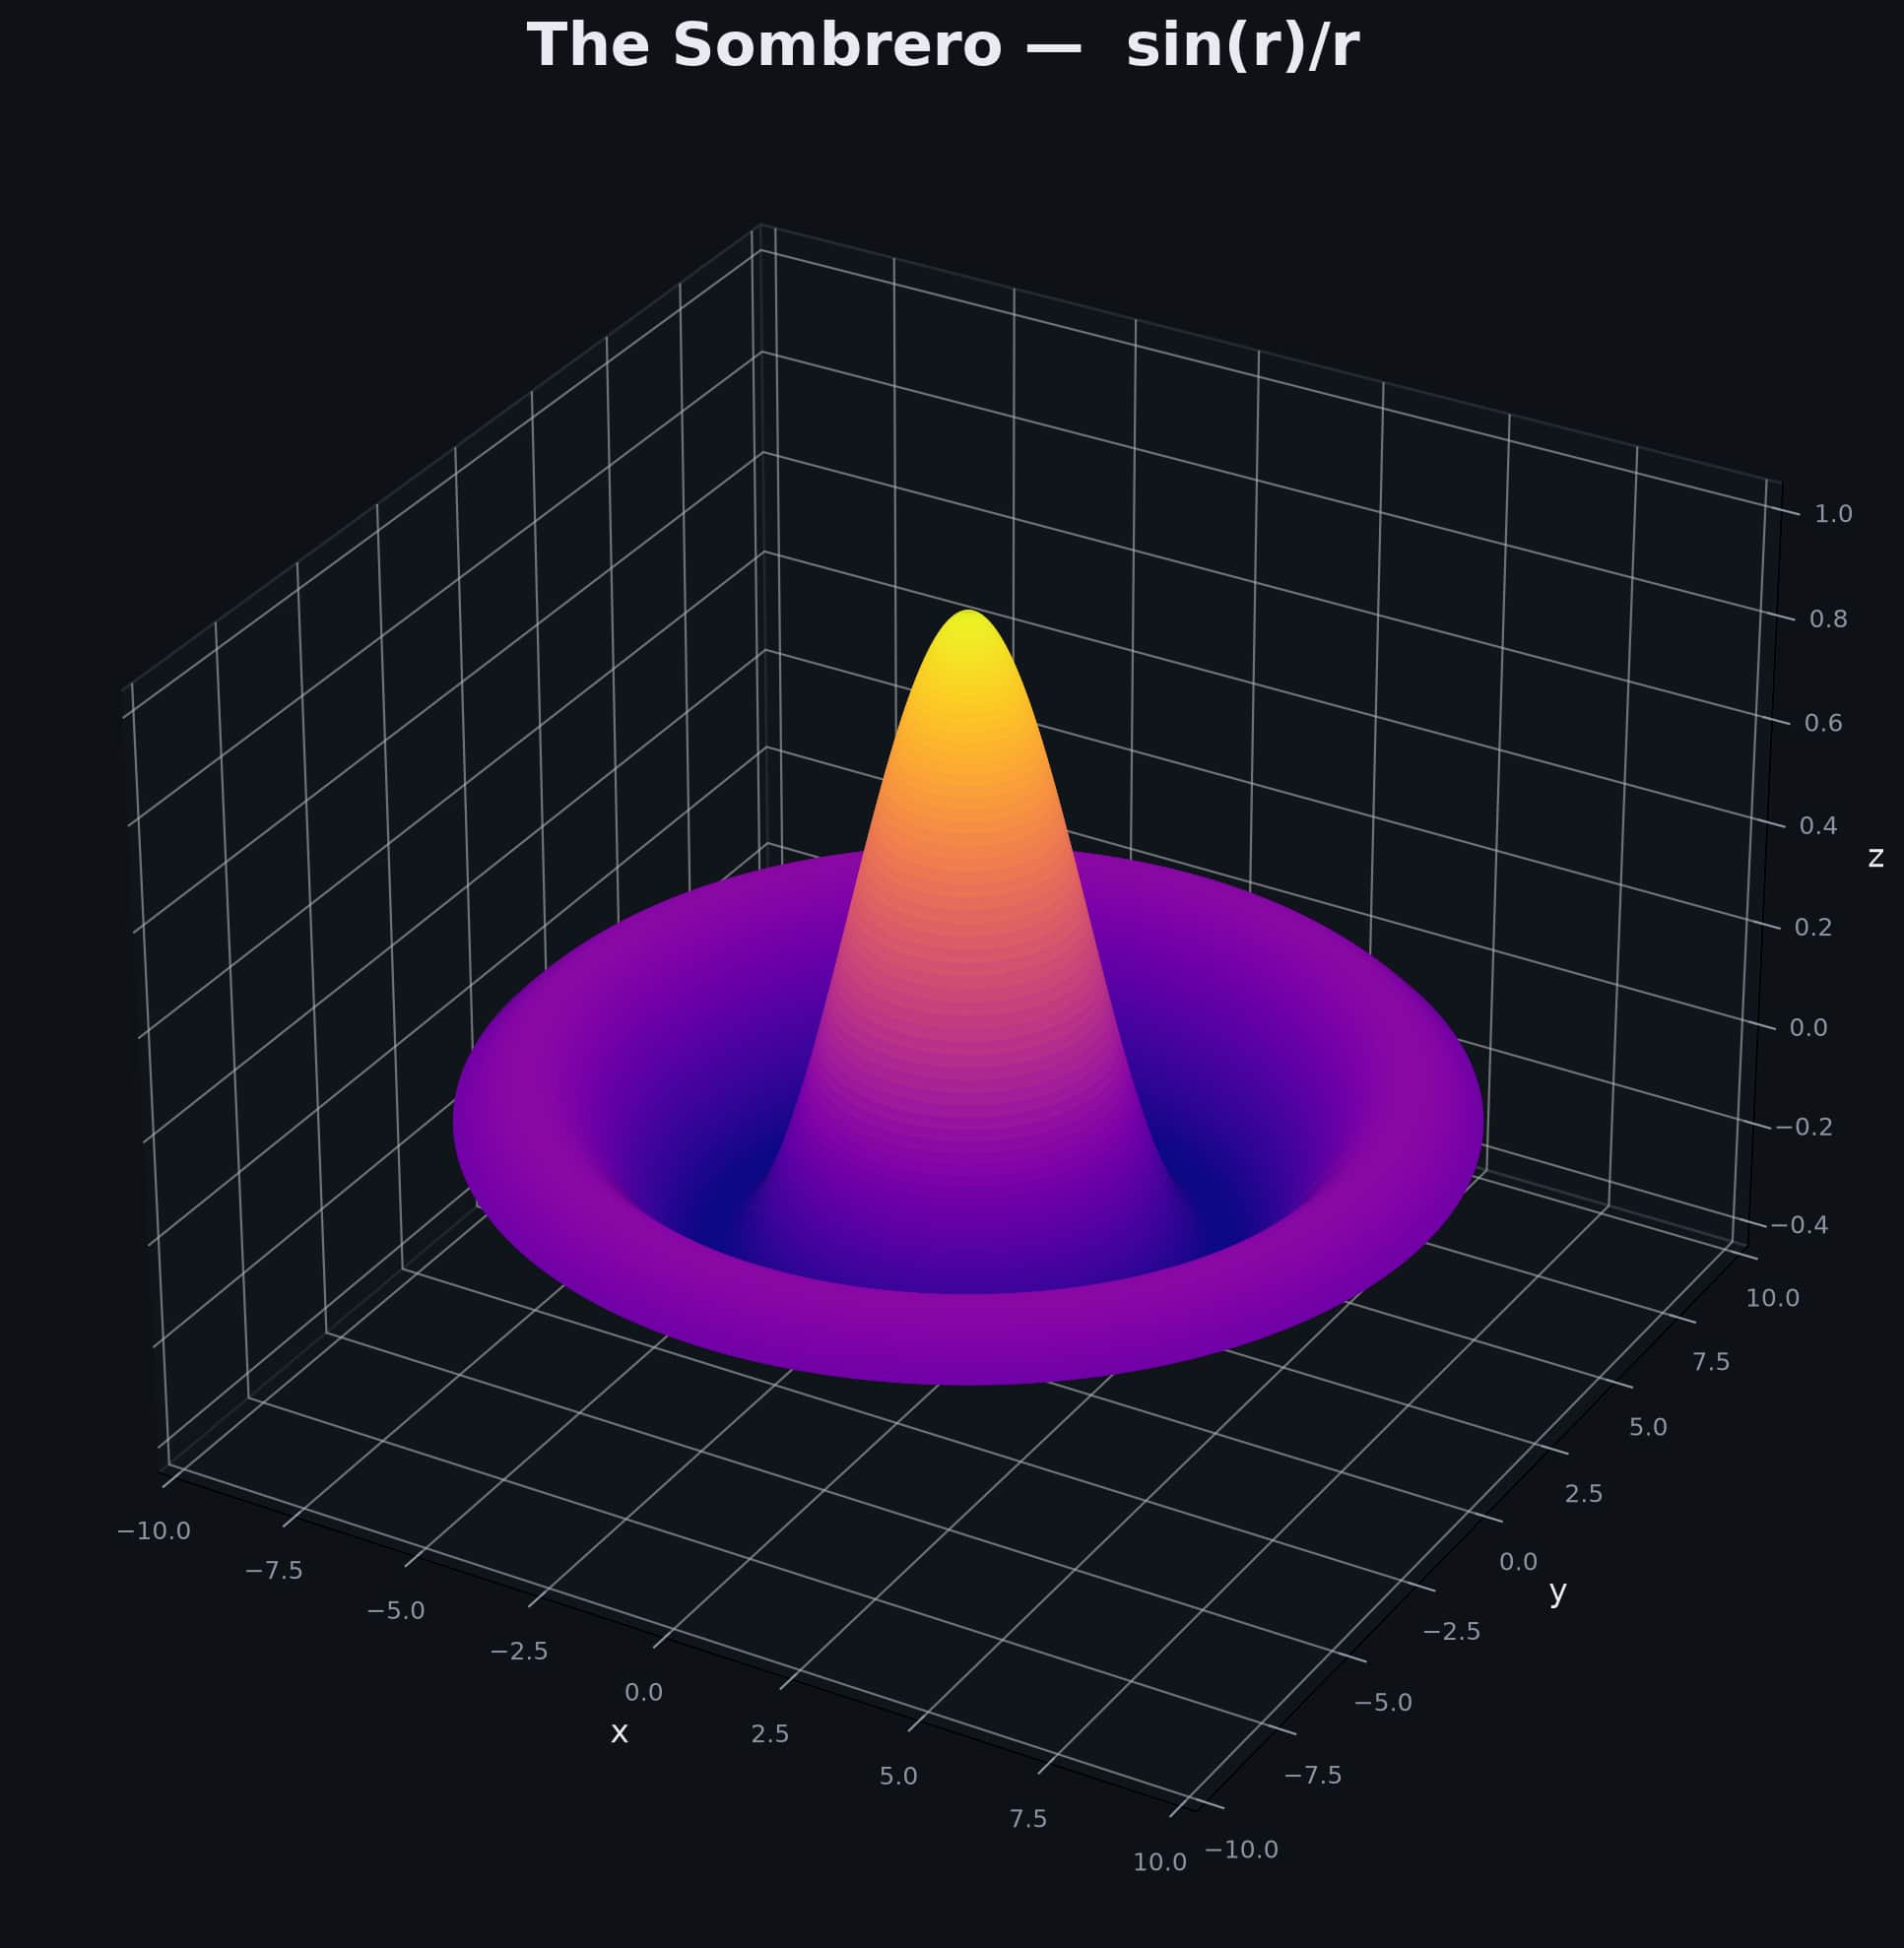
\includegraphics[width=0.85\linewidth]{graphs/sombrero3d}
	\caption{The surface of \cref{sombrero} over $x, y \in [-10, 10]$. The
	central peak is the removable singularity of \cref{series}; the circular
	trough around it is the first negative extremum of \cref{tab:extrema},
	swept through $2\pi$.}
	\label{fig:sombrero}
\end{figure}

One practical remark on evaluating either form numerically. Close to the
origin, $\sin r$ and $r$ are nearly equal, and computing their quotient in
floating point subtracts two almost identical quantities inside the sine
routine, so the result loses significant digits\footnote{The usual fix is to
switch to the truncated series of \cref{series} below some threshold, for
example $|r| < 10^{-4}$, where two terms are already accurate to machine
precision.}. This is the standard cancellation problem described in
\cite{numrecipes}, and it is worth guarding against before the plot rather
than after.

\clearpage
